Figure~\ref{fig:central_response_bias} summarizes the central response-fidelity bias comparison used in Table~\ref{tab:fidelitycentral}. Figure~\ref{fig:native_matched} shows the supporting native-versus-matched-transit control; it is included only to illustrate the sampling dependence discussed above.

\begin{figure}
\centering
\setlength{\unitlength}{0.8mm}
\begin{picture}(86,54)(0,0)
\put(15,10){\vector(1,0){66}}
\put(15,8){\line(0,1){4}}\put(15,4){\makebox(0,0){\scriptsize $-16$}}
\put(31,8){\line(0,1){4}}\put(31,4){\makebox(0,0){\scriptsize $-12$}}
\put(47,8){\line(0,1){4}}\put(47,4){\makebox(0,0){\scriptsize $-8$}}
\put(63,8){\line(0,1){4}}\put(63,4){\makebox(0,0){\scriptsize $-4$}}
\put(79,8){\line(0,1){4}}\put(79,4){\makebox(0,0){\scriptsize $0$}}
\put(79,10){\line(0,1){38}}
\put(1,42){\makebox(12,0)[l]{\scriptsize M0}}
\put(1,30){\makebox(12,0)[l]{\scriptsize M1}}
\put(1,18){\makebox(12,0)[l]{\scriptsize M2}}
\put(74.0,44){\circle*{1.8}}\put(73.9,40){\circle{1.8}}\put(82.7,36){\makebox(0,0){\scriptsize $+$}}\put(17.6,32){\makebox(0,0){\scriptsize $\times$}}
\put(78.9,32){\circle*{1.8}}\put(78.6,28){\circle{1.8}}\put(79.5,24){\makebox(0,0){\scriptsize $+$}}\put(65.8,20){\makebox(0,0){\scriptsize $\times$}}
\put(79.3,20){\circle*{1.8}}\put(78.9,16){\circle{1.8}}\put(79.3,12){\makebox(0,0){\scriptsize $+$}}\put(79.2,14){\makebox(0,0){\scriptsize $\times$}}
\put(18,50){\scriptsize $\bullet\ M_1\quad \circ\ M_2\quad +\ \varpi\quad \times\ \betag$}
\put(30,0){\scriptsize median fractional bias (\%)}
\end{picture}
\caption{Median fractional biases at the central response-fidelity point $\betag=0.25$, $\aalpha=1$, and $\psfelong=1.5$. The ordinary photocentre model produces coherent mass/parallax bias and a much larger light-fraction bias; the equal-width response removes most of the mass bias but retains measurable light-fraction error; the matched oriented response remains centered close to the injection.}
\label{fig:central_response_bias}
\end{figure}

\begin{figure}
\centering
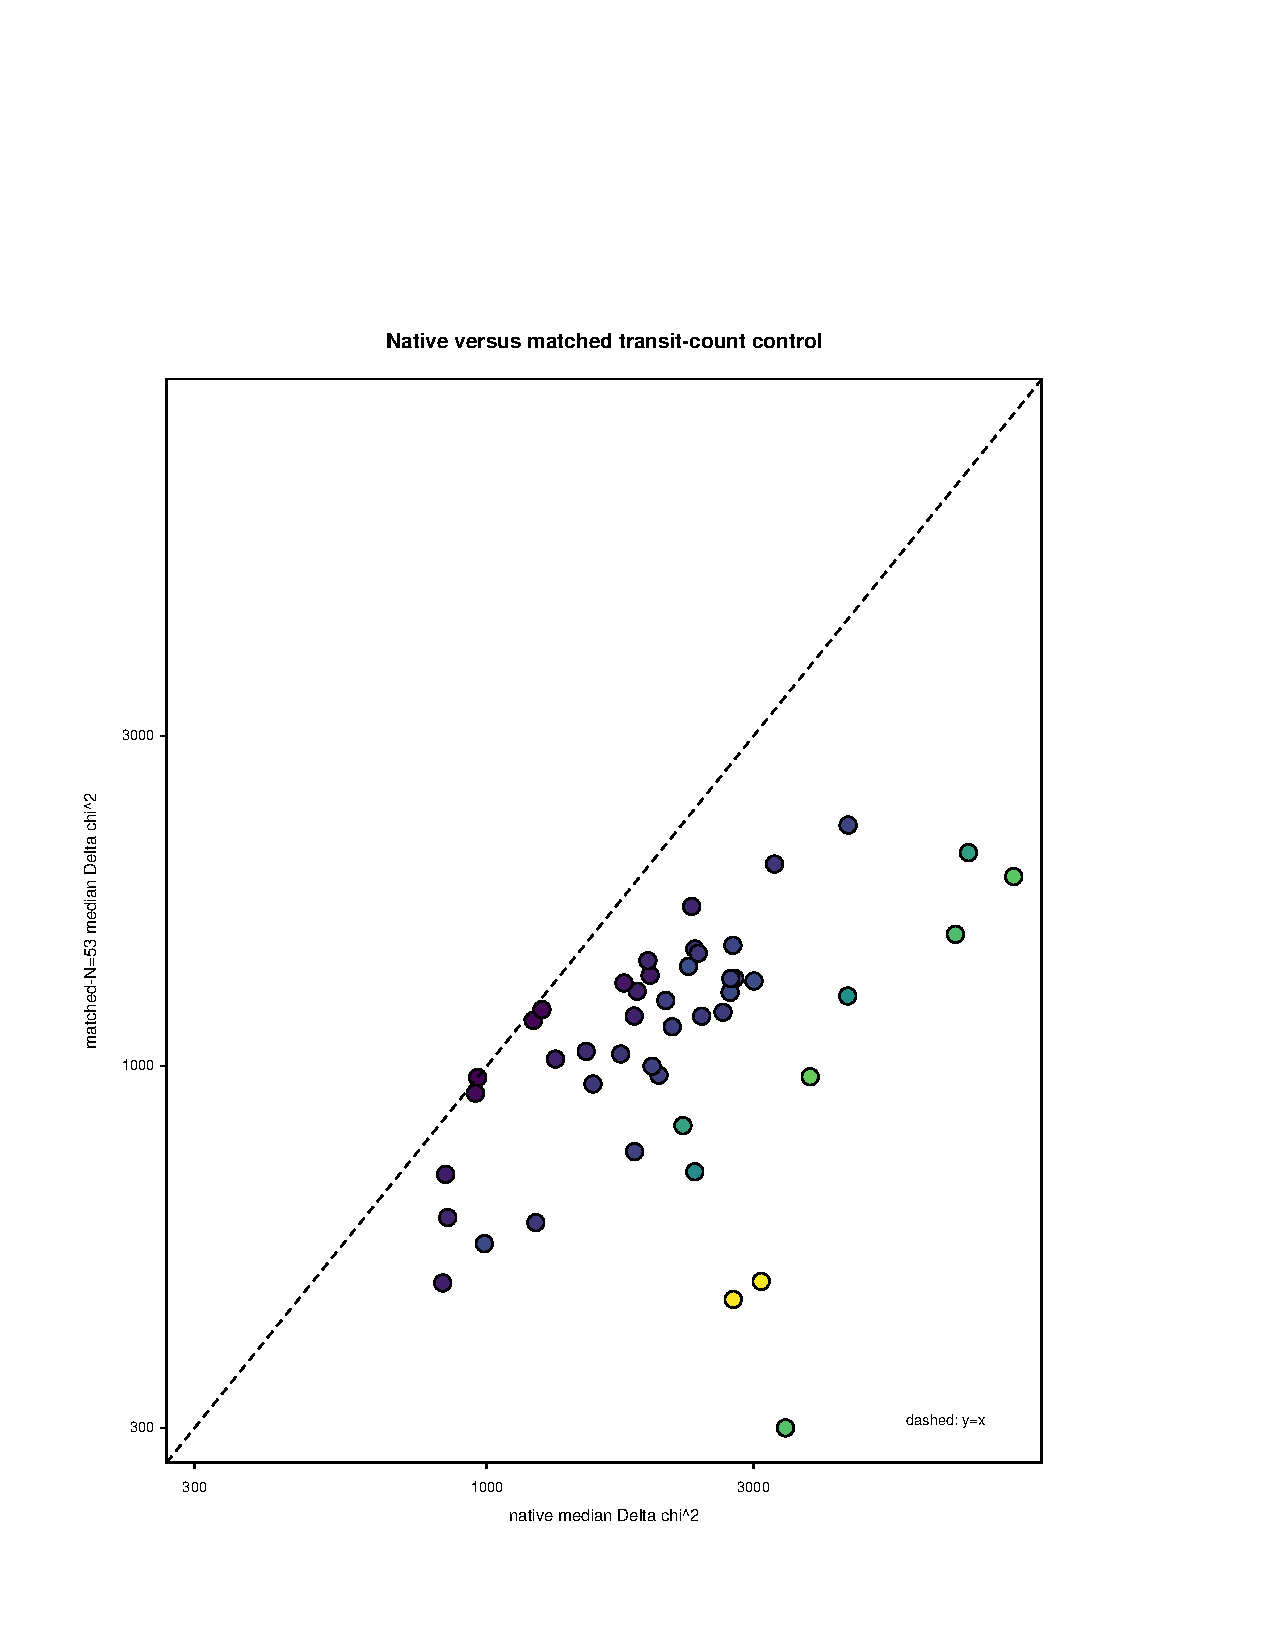
\includegraphics[width=0.96\columnwidth]{figures/full_sky_dr4_native_vs_matched_n53.pdf}
\caption{Supporting equal-width full-sky control comparing native nominal schedules with schedules matched to 53 transits per sky position. Equalizing transit count strongly reduces the apparent sky dependence of the accumulated photocentre mismatch, demonstrating that observation count and scan geometry must be separated when interpreting response detectability.}
\label{fig:native_matched}
\end{figure}
